\chapter{Analysis Overview}\label{ch:analysis_overview}

\section{The RPV UDD signature}\label{sec:signal_of_interest}

This analysis is a search for a supersymmetric partner to the gluon called the gluino, as described in~\ref{sec:susy_rpv}.
The process under consideration involves pair-produced gluinos decaying to a large number of standard model quarks via R-parity-violating decays.
In the direct decay model, each gluino decays directly to three standard-model quarks via an effective vertex with an off-shell squark propagator.
In the cascade decay model, each gluino first decays to a neutralino and two quarks, and the neutralino then decays similarly to three quarks vai the RPV effective vertex.
Both types of signal events would result in a large number of high-$p_{T}$ jets in the detector, because they have a large number of quarks in the final state, and each quark must be boosted due to the large mass of the gluinos.
Figure~\ref{fig:susy_rpv_decays} shows the diagrams for the two signal models under consideration.

\section{Run 1 limits}\label{sec:run1_limits}

A similar search was performed by ATLAS using $20.3~fb^{-1}$ of $8~TeV$ data, and limits were set on the gluino and neutralino masses~\cite{run1-multijet}.
For the cascade decay model, the observed limit on the gluino mass ranged from $800~GeV$ to $1~TeV$, depending on the neutralino mass.
Figure~\ref{fig:run1_cascade_limits} shows the $95\%$ CL lower bounds in the $(m_{\tilde{g}}, m_{\tilde{\chi}})$ plane from the search for the cascade-decay signal.
For the direct decay model, different limits were placed on the gluino mass for different assumptions about the flavor composition of the final states.
In the case of light-quark only decays, gluino masses above $917~GeV$ were excluded~\cite{run1-multijet}.

\begin{figure}[!ht]\centering
    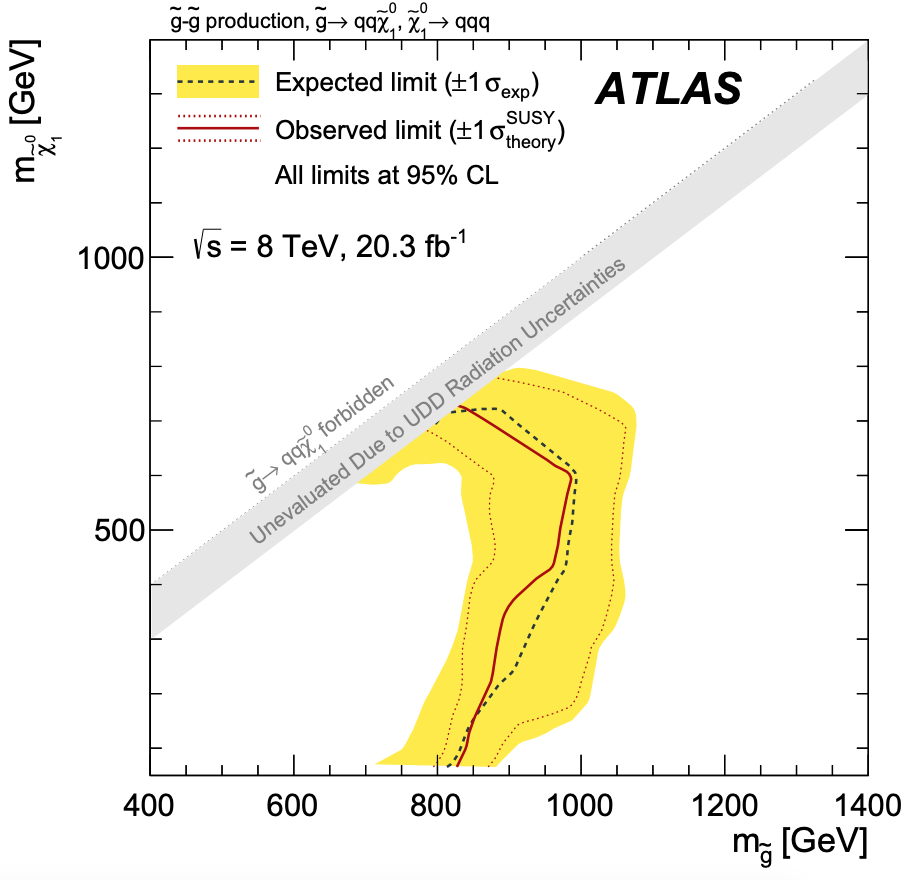
\includegraphics[width=0.6\textwidth]{analysis_run1_cascade_limits}
    \caption{Observed and expected limits in the $(m_{\tilde{g}}, m_{\tilde{\chi}})$ plane for the cascade-decay model in ATLAS Run 1 with $\sqrt{s}=8~TeV$~\cite{run1-multijet}.
    }
    \label{fig:run1_cascade_limits}
\end{figure}

\begin{figure}[!ht]\centering
    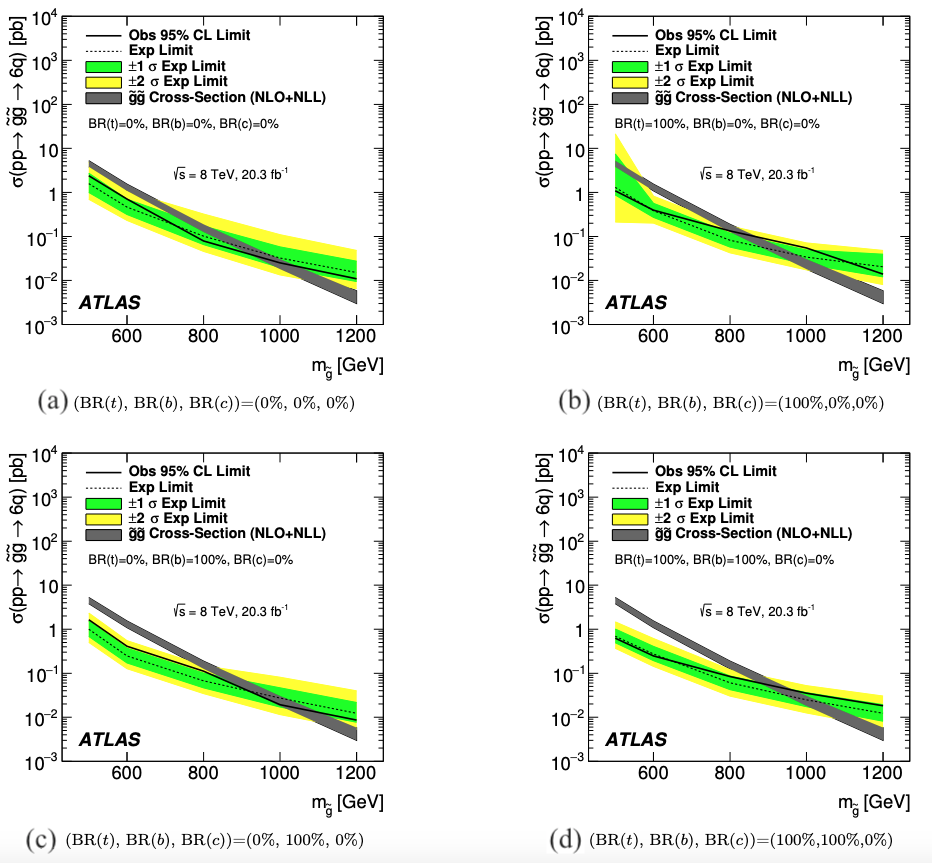
\includegraphics[width=0.6\textwidth]{analysis_run1_direct_limits}
    \caption{Observed and expected limits on $m_{\tilde{g}})$, along with theoretical cross-section for the direct-decay model in ATLAS Run 1 with $\sqrt{s}=8~TeV$~\cite{run1-multijet}.
    Different limits are set for four different branching fraction scenarios.
    In sub-figure (a), only light-quark decays are allowed.
    In sub-figure (b), each gluino decay results in a top quark in the final state.
    In sub-figure (c), each gluino decay results in a bottom quark in the final state.
    In sub-figure (d), each gluino decay results in both a top and a bottom quark in the final state~\cite{run1-multijets}.}
    \label{fig:run1_direct_limits}
\end{figure}

\section{Backgrounds}\label{sec:backgrounds}

\section{Search strategy and discriminating variables}\label{sec:search_strategy}

Two of the main discriminating observables, namely $M_J^{\Sigma}$ and $|\Delta\eta_{12}|$ are the same as those used in the Run-1 version of the analysis~\cite{run1-multijet}.
The first observable, $M_J^{\Sigma}$, is the scalar sum of the first four leading large-R jets, ordered by $p_{T}$, in an event.
Large-R jets have $R=1.0$ and are required to have $p_{T} > 200~GeV$ and $|\eta|<2.0$.
In case an event has less than four jets, the sum of all large-R jet masses passing the kinematic cuts is used.
$M_{J}^{\Sigma}$ provides good separation between signal and background because it takes into account both the energy and angular structure of an event, unlike a purely energy-dependent observable like $H_{T}$~\cite{hook-mj,elhedri-mj}.

The second discriminating variable is $|\Delta \eta_{12}|$, which is the pseudorapidity differences between the first two leading jets in an event.
Events with small $|\Delta \eta_{12}|$ have their leading two jets more central than average.
For regions with high jet multiplicity, requiring large $|\Delta \eta_{12}|$ reduces the signal to background ratio, allowing for the creation of high-multiplicity control and signal regions.
Distributions of the two discriminating variables are shown in figure~\ref{fig:MJ_dEta_distributions} for data as well as background and signal Monte Carlo.

\section{Discriminating variables}\label{sec:variables}
\begin{figure}[!ht]
    \centering
    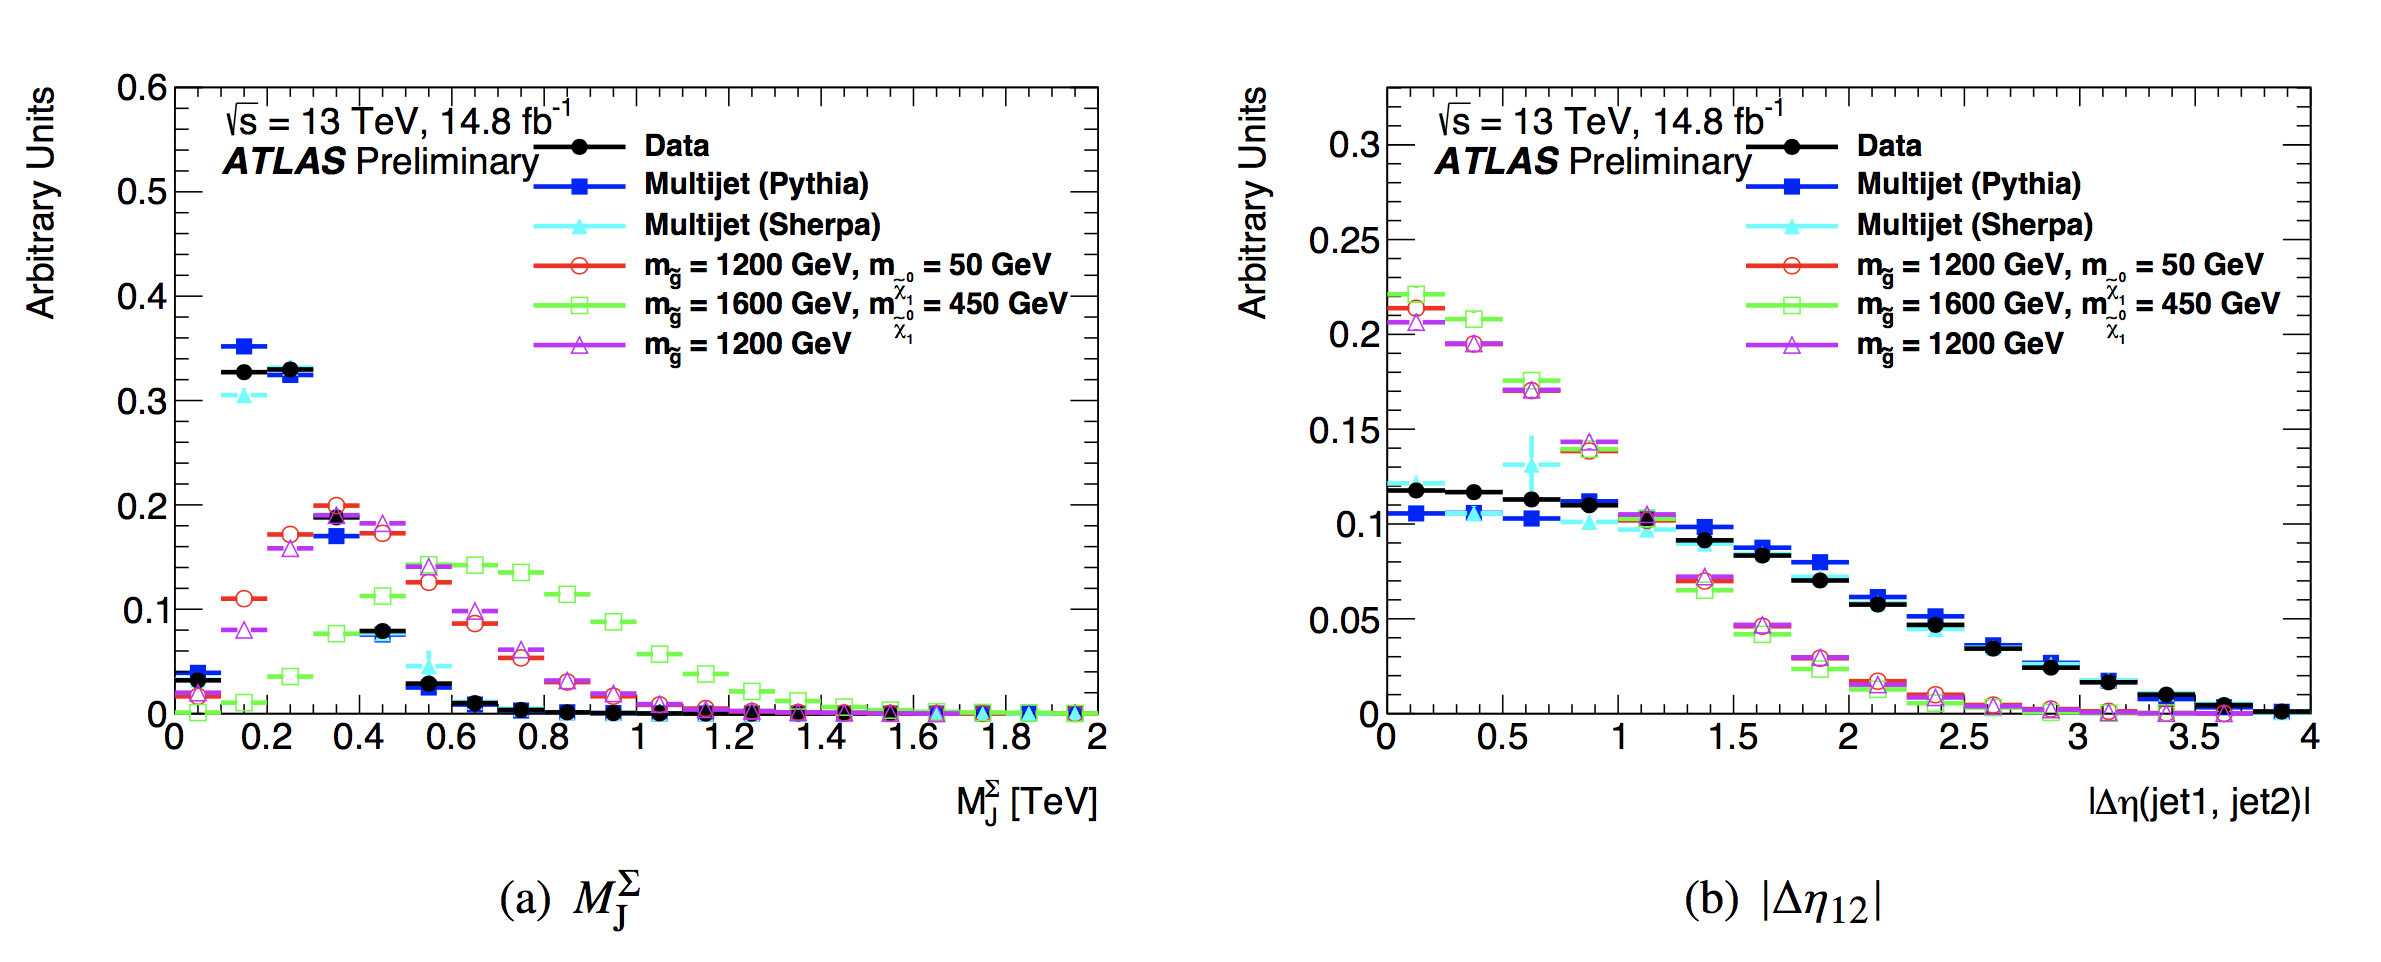
\includegraphics[width=0.9\textwidth]{MJ_dEta_distributions_combined}
    \caption{Distributions of the two main discriminating observables, (a) the scalar sum of the four leading large-R jets, $M_{J}^{\Sigma}$ and (b) the difference in pseudorapidity between the two leading jets, $|\Delta\eta_{12}|$.
    Selected events have $\geq 4$ large-R jets.
    Distributions are shown for both data and simulated signal and background samples.
    The red and green signal distributions are for the cascade decay mode, and the violet distribution is the direct decay mode, for the superpartner masses indicated~\cite{paper-plb}.}
    \label{fig:MJ_dEta_distributions}
\end{figure}




\begin{comment}
    


A data-driven method is used to predict the background yield in the signal regions, as well as the uncertainties on those predictions.
First, jet mass templates are created from control region jets.
Randomized jet masses, known as dressed masses, are generated from these templates for each jet in the kinematic sample.
Summing the dressed masses for each of the up to four leading jets in an event gives the dressed $M_{J}^{\Sigma}$ for that event.
The dressed $M_{J}^{\Sigma}$ distribution for each signal region is used to estimate the expected background contribution to that region.



A data-driven jet mass template method is used to estimate the background.
The method is similar to that used in the Run-1 version of the analysis~\cite{run1-multijet}, with a few important differences.

In the Run-1 analysis, the templates were smoothed with a kernel density estimate before sampling the dressed masses.
In this version of the analysis, the templates remain binned.
This allows for an estimate of the statistical uncertainty from the control sample size.
By Poisson fluctuating each template bin before sampling, the statistical uncertainty is propagated to the dressed $M_J^{\Sigma}$ distributions.

Secondly, in the Run-1 version of the analysis, two separate sets of templates were generated: one set for the leading two jets in each event,
and a separate set for the third leading jet.
In this analysis, the templates are instead divided into b-matched and non-b-matched jets.
The discrepancy in template shape between b-matched and non-b-matched jets was seen to be larger than that between the third leading jet and first two leading jets.

Finally, the Run-1 version of the analysis used Monte-Carlo non-closure as one contribution to the background systematic uncertainty.
In this analysis, a data-driven method is used instead.
This is due to the fact that the sample size of available simulated data was not large enough to make an accurate estimate of the non-closure.
\end{comment}